\documentclass{template/openetcs_article}
%\documentclass{article}
%\usepackage[ascii]{inputenc}
%\usepackage[T1]{fontenc}
\usepackage[english]{babel}
\usepackage{amsmath}
\usepackage{amssymb,amsfonts,textcomp}
\usepackage{array}
\usepackage{supertabular}
\usepackage{hhline}
\usepackage{graphicx}
\makeatletter
\newcommand\arraybslash{\let\\\@arraycr}
\makeatother
\setlength\tabcolsep{1mm}
\renewcommand\arraystretch{1.3}
\newcounter{Ilustracin}
\renewcommand\theIlustracin{\arabic{Ilustracin}}
\title{openETCS}

%\setcounter{tocdepth}{3}
\usepackage{float}
\usepackage{hhline}
\usepackage{booktabs}
\usepackage{multirow}
\usepackage{color, colortbl}
\definecolor{myblue}{rgb}{0.6,.6,1}
\definecolor{mydarkblue}{rgb}{0,0,0.5}
\definecolor{mylightblue}{rgb}{0.8,0.8,1}
\usepackage{hyperref}
\hypersetup{colorlinks=true, linkcolor=mydarkblue, urlcolor=mydarkblue}

\usepackage[textwidth=2.7cm,textsize=scriptsize,linecolor=green!40,backgroundcolor=green!40]{todonotes}

\newcounter{mycommentcounter}
\newcommand{\mycomment}[2][]
{
\refstepcounter{mycommentcounter}%
\todo[color={red!100!green!33}]{
\textbf{[\uppercase{#1} \themycommentcounter]:} #2}
}


\usepackage{lipsum,url}
\graphicspath{{./template/}{.}{./images/}}
\begin{document}
\frontmatter
\project{openETCS}

%Please do not change anything above this line
%============================
% The document metadata is defined below

%assign a report number here
\reportnum{OETCS/WP1/D1.3.1}

%define your workpackage here
\wp{Work-Package 1: ``Management''}

%set a title here
\title{Project Quality Assurance Plan - Review Process}

%set a subtitle here
%\subtitle{A template for short document. Adapted from report template.}

%set the date of the report here
\date{\today}

%define a list of authors and their affiliation here

\author{Ainhoa Gracia}

\affiliation{Avda. Zugazarte 8,6\\
  48930 Getxo \\
  Vizcaya, España}


% define the coverart
\coverart[width=350pt]{openETCS_EUPL}

%define the type of report
\reporttype{Description of work}




%=============================
%Do not change the next three lines
\maketitle
\tableofcontents
%\listoffiguresandtables
\newpage
%=============================

% The actual document starts below this line
%=============================


%Start here



%\begin{document}


\section*{Document History}

\begin{flushleft}
%\tablefirsthead{\hline Version & Date & Chapters modified & Reason & Name\\}

\tablehead{\hline \rowcolor{myblue} Version & Date & Chapters modified & Reason & Name\\}

\tabletail{}
\tablelasttail{}
\begin{supertabular}{m{1.1cm}m{1.8cm}m{2cm}m{7cm}m{2cm}lp{6cm}|}
\hline
0.0.1 &
24.05.2013 &
All &
First version &
SQS
\end{supertabular}
\end{flushleft}

\newpage

\section{Introduction}

\subsection[Introduction]{Purpose of the document}
This document presents the whole process to follow when documents need review. It aims to provide a set of guidelines as technical instructions to be used whenever a review process is ongoing, or there are a set of issues reported that shall be considered. The roles involved in the process are clearly identified as well as their responsibilities and tasks. And finally, the mechanisms needed to achieve the proposed objectives are also included, so the process can be carried out successfully.

\subsection{Intended Audience}
This document applies to the whole development life-cycle of the project and it addresses all the author(s)and reviewers involved. This document should be available to all of them in read access mode and it provides guidance about the Review process whenever it is needed. 

\subsection{Supporting documents}
\tablefirsthead{\hline
\rowcolor{myblue}
Name &
Path &
Contents\\}
\tablehead{}
\tabletail{}
\tablelasttail{}
\begin{supertabular}{|m{2cm}m{3cm}m{9cm}|}
\hline
Revision process &
governance/Review Process &
Presentation of the Revision process with details about the flow and technical instructions.
\\\hline
Revision and Review Processes summary &
governance/Review Process &
Brief presentation of the Revision process and the Review process as well as their interactions.
\\\hline
\end{supertabular}

\subsection{Definitions and acronyms}
\tablefirsthead{\hline
\rowcolor{myblue}
Abbreviation &
Meaning\\}
\tablehead{}
\tabletail{}
\tablelasttail{}
\begin{supertabular}{|m{3cm}m{11cm}|}
\hline
Revision Process &
The OpenETCS committers are invited to perform a revision of the contents of a document. The committers can edit the document, writing complete sections or making changes directly in it (LaTex, todonotes and Smartgit tools). The author(s) shall support the whole process answering questions and resolving conflicts. Once the author(s) and committers are satisfied with the results, the Product owner shall confirm and approve or reject and request more changes to the revised document. Finally, the approved document is pushed into the corresponding GitHub repository.
\\\hline
Review Process &
Any person involved in the GitHub communnity and/or the OpenETCS project is invited to participate in a Review Process. They shall not edit the document but send comments and suggestions creating the corresponding issues in the {\it Issue Tracker} tool. Once the deadline has arrived, the author(s) shall collect the comments and make the changes they consider appropriate. Any doubt shall be answered by the reviewers using the issue threads opened and in case of conflicts the collaboration of the Product owner may be required. The process may be launched after a Revision Process ends, there are relevant issues reported for a release or whenever the Product owner considers appropriate. 
\\\hline
Product owner &
The role played by the main author of a document or the project leader. The responsibilities of the role include launching a Review Process, inviting Reviewers to the process, closing discussions, taking decisions when there are conflicts and doing the final approval of the document among others.
\\\hline
Committer &
The role played by a member of the OpenETCS project who have been granted with this role by other committers and the project leader. There are some tasks that only can be done by committers such as: editing and pushing changes or new documents into a GitHub repository, closing of issues in the {\it Issue Tracker} or being involved in Revision processes.
\\\hline
Reviewer &
Any person of the community who is interested in providing feedback, reporting issues or propose improvements to a document. The reviewers can be involved in a specific Review process or open issues in an independent way. In any case they shall know the {\it Issue Tracker} tool to make their comments, be questioned by the Author(s) in case of doubts or be informed about the decisions taken regarding the implementation or not of changes due to the issues found.
\\\hline   
\end{supertabular}

\section{Tools}

\begin{flushleft}

\begin{tabular}{|m{3cm}|m{11cm}|}
\hline
\rowcolor{myblue}
\multicolumn{2}{|c|}{Tools} \\\hline
GIT &
\begin{itemize}
\item \underline{GitHub}: A web-based hosting service for projects that use Git revision control system.
\item \underline{Issue Tracker (in GitHub)}: The issue tracker is integrated with the project's repository. Some of the features included are: the possibility of modifying tickets from within commit messages,
creating and applying labels to issues to assign to users or categorize, voting on issues that you want to see tackled, searching, sorting, and filtering, and keyboard shortcuts.
\end{itemize}
\\\hline
PDF documents &
\begin{itemize}
\item \underline{Adobe Acrobat Reader}: Software package that allows to view, navigate and print pdf files.
\item \underline{Diffpdf}: Open source application that compares different PDF files for discrepancies. 
\end{itemize}
\\\hline
\end{tabular}
\end{flushleft}

\section{Review Process overview}
\subsection{Structure of the repository}
 
There is no need of additional working directories for a Review process, considering no branches shall be created and the changes to be included in a version of a document shall be minor changes.

\subsection{Review Roles}

This section describes the roles of the participants in the review process of a document:

\begin{flushleft}
\begin{tabular}{|m{3cm}|m{11cm}|}
\hline
\rowcolor{myblue}
\multicolumn{2}{|c|}{Roles} \\\hline
\rowcolor{lightgray}
Role &
Competencies \\\hline
Product owner (main author or project leader) &
\begin{itemize}
\item Launch the Review Process when it applies
\item Notify the Community with a new issue in the {\it Issue Tracker} that the document is under Review and Reviewers are invited to collaborate ({\it TI.1.1. Create e New Issue})
\item Control Review Process 
\begin{itemize}
\item Approve the reviewed version and confirmation of changes made 
\item Propose a new Revision process due to further improvements are needed 
\item Send the notification of closing. 
\item Generate an established version of the document and pushed it in the corresponding GitHub repository. ({\it LaTex and PDF versions})
\end{itemize}
\end{itemize}
\\\hline
\end{tabular}
\end{flushleft}

\begin{flushleft}
\begin{tabular}{|m{3cm}|m{11cm}|}
\hline
\rowcolor{myblue}
\multicolumn{2}{|c|}{Roles} \\\hline
\rowcolor{lightgray}
Role &
Competencies \\\hline
Author(s) & 
\begin{itemize}
\item Issues collection. 
\begin{itemize}
\item Collect all the issues once the deadline of an ongoing Review process arrives 
\item When there is not a Review Process launched, check the {\it Issue Tracker} periodically to see whether there are new issues to be considered.
\item Analyse the reported issues and decide what implementations and changes are needed. In case of doubts ask questions to the Reviewers in the {\it Issue Tracker} ({\it TI.1.2 Add comments in the Issue Tracker})
\end{itemize}
\item Editing the document
\begin{itemize}
\item When there are conflicts or discussions not solved, require the involvement of the Product owner to close the pending issues. 
\item Make changes to the document when needed using editing tools (LaTex editing tools, pdf generation tools).
\end{itemize}
\item Closing of the Review Process or collected issues
\begin{itemize}
\item Close the issues made by the reviewers 
\item Make a request to the product owner for a final confirmation of the Review process. 
\end{itemize}
\end{itemize}
\\\hline
\end{tabular}
\end{flushleft}

\begin{flushleft}
\begin{tabular}{|m{3cm}|m{11cm}|}
\hline
\rowcolor{myblue}
\multicolumn{2}{|c|}{Roles} \\\hline
\rowcolor{lightgray}
Role &
competencies 
\\\hline
Reviewers &
\begin{itemize}
\item Confirm the participation in an ongoing Review adding a comment to the Review Process opening issue. ({\it TI.1.2 Add comments in the Issue Tracker}). In any other case, the Reviewer shall open a new issue identifying clearly the document he/she is reviewing. ({\it TI.1.1 Create a New Issue})
\item Involve the author(s) whenever it is necessary asking questions and resolving doubts.
\item Try to group similar issues under the same message in the {\it Issue Tracker}, put a label to each reported issue (bug, enhancement, question) to help the Author(s) to group issues when collecting them.
\item Before publishing an issue, be sure there are not other issues that are reporting the same subjects.
\end{itemize}
\\\hline
\end{tabular}
\end{flushleft}

\subsection{Description of the Review Process}

The documents review process aims to collect verifiable data and information in an independent way, and the process provides an overall improvement of the contents and/or format of the document, so accurate and up-to-date documents with increased credibility are obtained.

The Review process allows the OpenETCS project to ensure that the information contained in a document is independently verifiable. The process can be done without needing to solicit extensive input
from other sources and it is typically less expensive than collecting the data using other methods.

The objectives to accomplish in any Review are the following ones:

\begin{itemize}
\item Evaluate the next aspects
\begin{itemize}
\item Accuracy
\item Completeness
\item Conciseness
\end{itemize}
\item Reduce the defect percentage
\item Improve the quality of documents
\begin{itemize}
\item Focus on correcting the defects
\end{itemize}
\end{itemize}

To accomplished a successful process the role of the participants shall be clear and their involvement active. This document will help the reviewers to understand their roles and
activities to practice effective and efficient reviews; and on the other hand, the author(s) to comprehend the importance of checking periodically the {\it Issue Tracker} tool to answer the reviewers as soon as possible, so they feel attended and their feedback valued.

The reviewers shall verify technical details and could share their vision with other reviewers participating in different discussions held in the {\it Issue Tracker}. 

The Review shall be focused on the work product and whenever additional help is needed the Author(s) shall be available to answer questions. Only in case there are conflicts or no agreements are reached, the Product owner shall be required to close the pending issues.

Finally, the Product owner shall evaluate the state of the document once the Review has finished and decide whether the new version deserves a new release for the document, or it is rejected due to minor changes still pending to be implemented (The review process continue) or further improvements are identified and a Revision process needs to be launched to modify the document accordingly.

The Review Process refers to documents that are prone to be under review consideration because:

\begin{itemize}
\item After a Revision Process has finished
\item There is a release of a document and in the {\it Issue Tracker} there are a set of relevant issues to that release. A Review process shall be started to collect more issues.
\item There is a special situation because of that the Product owner considers to begin a Review Process 
\end{itemize}

The following diagram provides a general overview of the process. 

\begin{figure}[H]
\centering
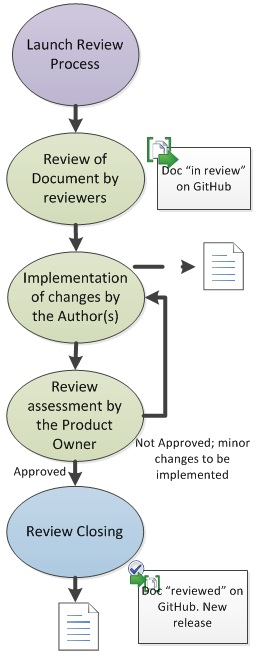
\includegraphics{./figures/ReviewProcess.JPG}
\caption{Review Process flow}
\end{figure}

During their lifetime, these documents shall be involved at least in one complete Review Process, but it there will be as many Review Processes launched as considered necessary.    

The process is divided in the following stages

\subsubsection{Review Process Launching}

Having the document reviewers work together from a shared space (GitHub {\it Issue Trucker}) increases productivity and accuracy. They can ask questions as they come up and the author(s) can give the answers to all reviewers at once.

The reviewers can participate in a review in two different ways:

\begin{itemize}
\item The product owner of a document launches a Review Process creating an issue in the {\it Issue Tracker}. The issue shall contain basic information about the document, the objectives to accomplish, and the deadline. Any person of the community is invited to participate, so the reviewer only has to answer the issue indicating his/her interest in collaborating.
\item There is not an ongoing Review Process for a document, but a person who has read a document has found some issues he/she wants to report. The reviewer can open a new issue in the {\it Issue Tracker} to notify the findings; depending on the severity and category of the defects detected or improvements identified, the Product owner can decide to open a Review Process, or directly ask the author(s) for implementing the appropriate changes without launching the process.
\end{itemize}

The document shall be available in a readable format (PDF) so any reviewer can have access to it, and the correctly path to download it shall be provided.

The launching of the Review process shall consist on the following steps:
\begin{itemize}
\item The Product owner should assess whether there are any specific reviewer he/she is interested in inviting due to his/her knowledge in an area. In this case, the Product owner shall notify personally via e-mail the opening of the Review Process and the invitation to collaborate.
\item Specify a deadline for the Process.
\item The Product owner shall be the responsible for addressing and conducting the main aspects of the Review. 
\begin{itemize}
\item The critical decisions regarding the process shall be taken by this role (closing of issues when no agreements have been reached and conflicts solving).
\item But the process itself shall be mainly supported by the Author(s), so any problem, doubt or question the reviewers have about the process or contents of the document must be asked to the Author(s) using the {\it Issue Tracker} tool. 
\item The Product owner shall be aware of the progress of the Review, so it is under control. 
\end{itemize}
\end{itemize}

From this moment, the last version of the document that can be a \underline{Revised document} or a \underline{Released document} is put {\it \underline{In Review}}.

\subsubsection{Review Stage}

Any person involved in the community and the OpenETCS project can be a reviewer at any time, when there is a Review process launched, and when it is not.

\begin{itemize}
\item In case there is a Review process ongoing, the difference is that the Reviewers shall consider the deadline defined for reporting issues, and in that time, they can share their findings and promote discussions so the best solution for a problem is agreed. 
\item In case there is not a Review process launched, the reviewer shall wait for the Author(s) to answer the issue(s) reported and decide whether they shall be considered and a solution implemented or not. In any case, the Author(s) shall justify their decision.
\end{itemize}

The Author(s) shall be aware about the issues and be available to answer the questions asked during the discussions between different reviewers or provide support to a specific reviewer when required.

On the other hand, the Reviewers shall also check the {\it Issue Tracker} to read the answers provided by the Author(s) or clarify their doubts regarding the issues found.

The only tool available during the Process is the {\it Issue Tracker} available in GitHub. The Reviewers are responsible for learning its functionalities and options and being sure they do an appropriate use of it.

It is highly recommended the Reviewers group the issues found in categories by similarity and report each group in a different issue. In this way, the issues shall be easier to follow and assess and the  {it Issue Tracker} more organised.

When the document under review is an intensive or complex one, or there is a considerable number of questions or doubts between the Reviewers, the Product owner or the Author(s) can propose online meetings to solve them.  

By defect, the period of time for the Review Stage must not exceed two weeks.

The stage implies the following \underline{key points}:

\begin{itemize}
\item The Reviewers shall communicate to the Author(s) their interest in participating in an opened Review Process adding a comment to the corresponding issue. 
\item The {\it Issue Tracker} shall be the main tool to make comments and suggestions, as well as receive answers and discuss subjects.
\item The issues must be labelled, so the Author(s) can prioritize them and organize the Stage of implementation.
\item The Reviewers shall check there are not other issues reported that deal with the same subjects they want to publish.
\end{itemize}

\underline{A successful Review lies in}:
\begin{itemize}
\item The Reviewers' ability to communicate issues as well as their ability to collaborate with the Author(s) or other Reviewers. 
\item The Reviewers have in mind the deadline in case there is a Review Process and they do the review in the period established.
\item Whenever it is necessary the Reviewers shall ask for support from the Author(s)
\end{itemize}

\subsubsection{Implementation Stage}

Once the deadline arrives in a Review process launched, or there are some issues reported in the {\it Issue Tracker} that have been considered as adequate, the Implementation Stage begins.

The Author(s) shall be the responsible for collecting the issues reported in the {\it Issue Tracker} organising and prioritizing them so they can assess whether new implementations or changes are needed.

During a specify period of time (approximately one week), the Author(s) shall implement the changes, contact the Reviewers in case of doubts, and inform the Reviewers when the Implementation phase has finished.

The Author(s) shall prepare a new version of the document and push it into the corresponding GitHub repository. They shall inform the Reviewers they have a couple of days to make comments to that version so minor adjustments can be done and then the Stage shall be closed.

The Author(s) are responsible for using the appropriate editing tools to include the changes as well as providing a correct upload of the new version to the repository.

\subsubsection{Approval Stage}

Now that the Review stage is completed, the Approval stage begins. 

During this stage, the \underline{Product owner} can resolve duplicate or
conflicting information and requests. He/she shall be required to assess the state of the document, so the Author(s) shall provide a list of the issues reported, a list of the issues implemented and the last version of the document to the Product Owner.

If required, more information can be requested from the Author(s) or Reviewers about a
particular aspect of the Review. 

The Product Owner shall evaluate carefully the Review of the document, the changes made and the current contents. Then The Product owner shall decide:

\begin{itemize}
\item To Approve the document
\begin{itemize}
\item The document satisfies the expectations, the contents are good and the changes made appropriate. 
\item The Approval stage finishes and the Product owner makes the closing.
\end{itemize}
\item The document still have minor defects, errors or improvements. The Product Owner shall notify the Author(s) the changes he/she require(s) and provide a deadline for the implementation. After that, he/she shall analyse again the state of the document and decide whether it deserves to be approved or not.
\item There are pending issues that cannot be resolved in a Review or further improvements are needed. The Review has found that the structure, main contents or several sections need a deep Revision. In this way, the Product owner closes the Review notifying it to the Reviewers (in the Review issue or personally in each issue reported in the {\it Issue Tracker} and launches a complete \underline{Revision Process} to involve committers.
\end{itemize}

Whatever decision is made, it shall be justified by the Product owner and communicated to the Author(s) and Reviewers.

\subsubsection{Closing}

A Review process or a review made by one or more Reviewers without a Review process shall be closed when:

\begin{itemize}
\item The document review has been approved
\item The document shall be revised deeply by the Committers and the Author(s), so the Review shall be closed and another Review opened once the new Revision is done.
\end{itemize} 

In case the document has been approved, the Product owner prepares the version (in LaTex and PDF) and pushed both documents to GitHub with the appropriate version numbering. This document shall be available as a \underline{Release}.

In any case, the Product owner shall close the corresponding issue in the repository (if it exists) or confirming the closing adding comments to each issue reported. 

\section{ANNEXES - Technical Instructions for using the Issue Tracker tool}

In this section the whole Review process is explained using technical instructions, so all the participants involved in the process are aware of the main mechanisms the tool selected for supporting the Review have. 

\subsection{Create a New Issue}

\begin{flushleft}
\tablefirsthead{}
\tablehead{}
\tabletail{}
\tablelasttail{}
\begin{supertabular}{|m{2cm}|m{13cm}|}
\hline
\rowcolor{myblue}
TI & 
TI.1.1. Create a New Issue
\\\hline
Roles &
Product owner, Reviewers
\\\hline
Description &
A new issue shall be opened whenever a set of defects, errors or improvements want to be reported to the Author(s) of a document.
\\\hline
Steps &
\begin{itemize}
\item Create a new issue in the repository that contains the document under review. 
\begin{enumerate}
\item Open Github and go to the appropriate repository
\item Select the {\it Issues section}
\item Push the {\it New issue} button
\item Add a descriptive title indicating the name of Document under Review
\item Provide the contents of the issue
\begin{itemize}
\item The issue is created by the Product owner referring a new Review process: the deadline, the objectives and the expectations
\item The issue is created by a reviewer: explain in detail the problem, defect or improvement identified, and if it applies, propose a solution. In case there is a Review Process be sure the issue is posted before the deadline.
\end{itemize}
\item Push {\it Submit new issue}
\end{enumerate}
\item The Product owner shall notify the opening of the issue personally to the reviewers he/she want to participate. 
\end{itemize}
\\\hline
\end{supertabular}
\end{flushleft}


\subsection{Add comments in the Issue Tracker}

\begin{flushleft}
\tablefirsthead{}
\tablehead{}
\tabletail{}
\tablelasttail{}
\begin{supertabular}{|m{2cm}|m{13cm}|}
\hline
\rowcolor{myblue}
TI & 
TI.1.2 Add comments in the {\it Issue Tracker}
\\\hline
Roles &
Product owner, Author(s), Committers
\\\hline
Description &
Adding comments to an issue is needed whenever a discussion or a notification is required. In any case or context, the people involved in a Review Process shall need to add comments to an opened issue.
\\\hline
Steps &
\begin{itemize}
\item Go to the repository where the document under Review is located.
\item Select the issue that refers to the document under Review.
\item The comments posted shall be descriptive enough so any reader can understand the message. 
\begin{enumerate}
\item Identified yourself clearly, providing your name and role in the project.
\item When required, include diagrams, figures, partial texts or specific data that help to understand the problematic found.
\end{enumerate}
\item Do not edit any comment done. It is a better option to rewrite it with the additions you proposed than editing and make the changes directly. In this way, it is assured that everyone reads the new message because in the other case, the change/addition can be missed.
\item Push the {\it Comment} button to post the message.
\end{itemize}

\\\hline
\end{supertabular}
\end{flushleft}

\subsection{Closing an issue}

\begin{flushleft}
\tablefirsthead{}
\tablehead{}
\tabletail{}
\tablelasttail{}
\begin{supertabular}{|m{2cm}|m{13cm}|}
\hline
\rowcolor{myblue}
TI & 
TI.1.3 Closing an issue
\\\hline
Roles &
Product owner, Author(s)
\\\hline
Description &
Once a Review Process has finished, or an specific issue reported by a Reviewer has been considered (accepted or not) a closing is needed so the issue do not appear as pending in the {\it Issue Tracker}
\\\hline
Steps &
\begin{itemize}
\item The product owner or the Author responsible for closing the issue(s) shall have the appropriate permissions to close issues in the repository. Mainly he/she shall have the role of Committer. Because of this, in case he/she has not got the required rights, he/she shall contact the Project leader to discuss the convenience of modifying the assigned permissions or assigned a person who are in charge of this task.
\item Select the issue to close.
\item Add a comment notifying the closing and justifying it: the issue has been considered and changes implemented, the issue has been rejected because it does not apply, the issue to close is the issue that informs the opening of the Review Process and it has finished, etc.
\item Push the {\it Close \& Comment} button
\item Confirm in the {\it Issue Tracker} that the issue has been closed correctly.
\end{itemize}

\\\hline
\end{supertabular}
\end{flushleft}

\end{document}
